\documentclass{article}


\usepackage{graphicx}
\usepackage{hyperref}
\usepackage[utf8]{inputenc}
\usepackage[francais]{babel}


\title{De Révolution à Evolution \\ Création d'un jeu vidéo sur les thèmes de l'écologie et de la transition énergétique}
\date{16-02-2018}
\author{Niels Lachat \\ Mentor : Patrick Rickli}

\begin{document}
        \pagenumbering{gobble}
        \maketitle
        \newpage

        \tableofcontents
        \newpage
        \pagenumbering{arabic}

        \section{Introduction}
        Le but de ce travail de maturité était de créer un jeu vidéo abordant les thématiques de l'environnement et de la transition énergétique. 
        Le genre du jeu de gestion a été choisi pour démontrer les principes économiques de la transition énergétique.
        Ces principes ont bien entendu été simplifiés et modélisés afin de pouvoir les intégrer dans un jeu vidéo.
        \\
        Je présenterai tout d'abord le concept sur lequel le jeu a été basé et j'expliquerai ensuite comment le joueur interagit avec le jeu.
        Je conclurai par une explication du fonctionnement d'une partie du code du jeu.

        \section{Concept du jeu}
        \subsection{Développement du concept}
        
        Initialement, mon projet était de créer un jeu de gestion de ressources dont l'univers du jeu était aussi proche que possible de la réalité. Je me suis rapidement rendu compte que je devrais faire des simplifications pour que le jeu soit intéressant à jouer et que le projet soit réalisable avec le temps que j'avais à disposition. \\
        La mécanique économique étant la mécanique principale de jeu, il était primordiale qu'elle soit bien pensée.
        
        \paragraph{Première } \hspace{0pt} \\
        

        \subsection{Concept final}

        \section{Le jeu}
        \subsection{Interaction du joueur}

        \subsection{Fonctionnement du jeu}
        
        \section{Conclusion}

        \begin{figure}[h]
                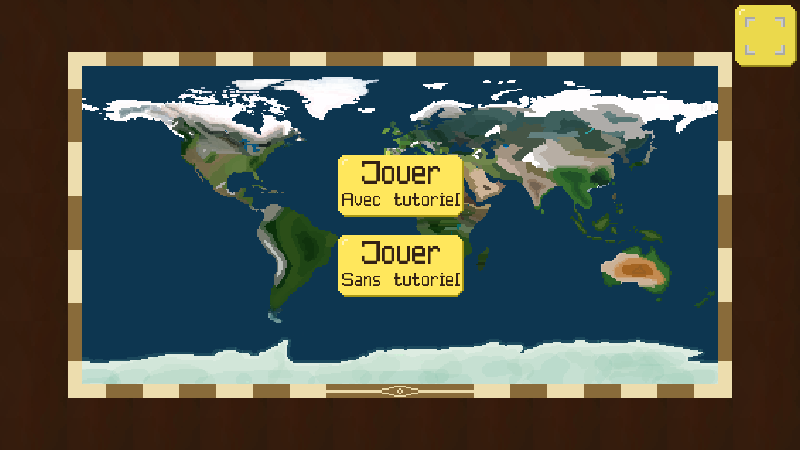
\includegraphics[width=\linewidth]{../images/mainMenu}
                \caption{Menu principal du jeu}
                \label{fig:mainMenu}
        \end{figure}

        Figure \ref{fig:mainMenu}

        \href{https://www.latex-tutorial.com/tutorials/pgfplots/}{Lien vers le tuto}



\end{document}
